    
\chapter{Koncepcja rozwiązania} \label{chap:methodology}

\section{Opis problemu}
\label{sec:problemDescription}
Problemem do rozwiązania dla zaimplementowanego systemu będzie podejmowanie decyzji w związku z wartościami parametrów produkcji odlewanego detalu biorąc pod uwagę:
\begin{itemize}
    \item spełnienie wymaganej jakości dla danego zamówienia,
    \item uzyskanie jak najmniejszego kosztu produkcji,
    \item zwiększenie wiarygodności parametrów zwracanych przez system na podstawie preferencji użytkownika.
\end{itemize}

Wymaganą jakość dla danego zamówienia określa norma EN-PN 1564:2012 \cite{pnen1564} (rys. \ref{fig:en-pn-1564}). Zawarte są w niej właściwości fizyczne stopów ADI w odniesieniu do oznaczeń, jakie są używane w przekazywanych informacjach między odlewnią a jej klientami.
\begin{figure}[ht]{}
	\centering
	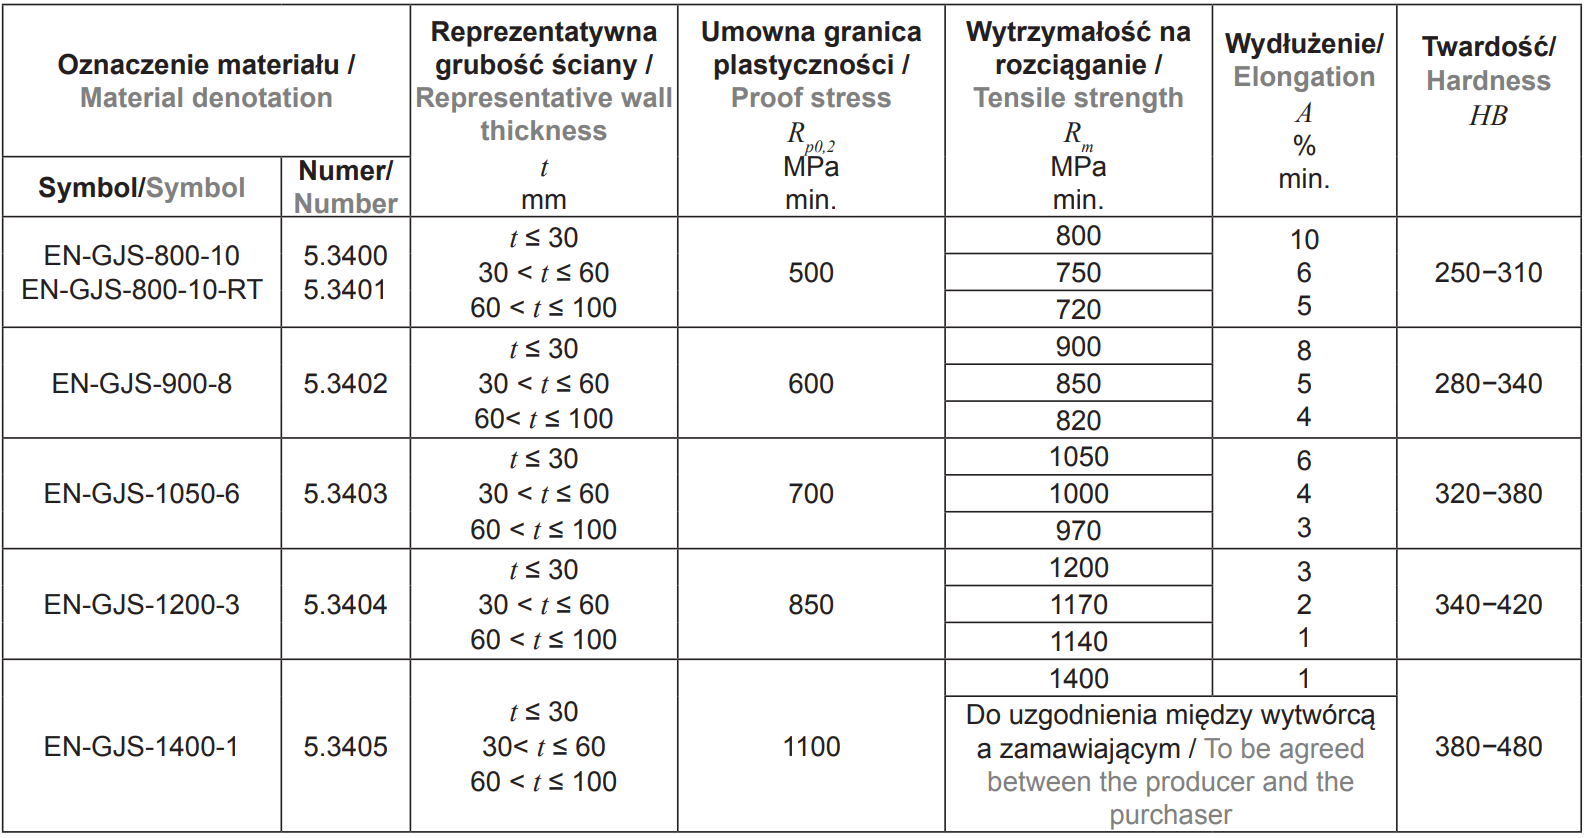
\includegraphics[scale=0.35]{images/en-pn-1564.PNG}
	\caption {
		 Właściwości mechaniczne żeliwa ADI wg PN-EN 1564:2012.
	}
	\label{fig:en-pn-1564}
\end{figure}

W celu lepszego zrozumienia sposobu pracy odlewni zostały sporządzone diagramy obrazujące w uproszczony sposób jak wygląda proces produkcji w takim zakładzie (rys. \ref{fig:schemat_linii}).
\begin{figure}[ht]{}
	\centering
	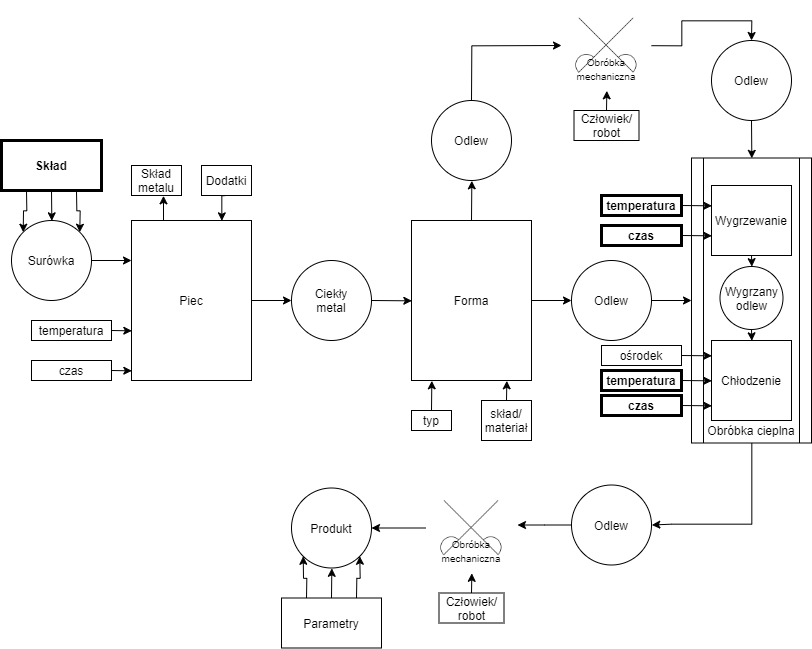
\includegraphics[scale=0.4]{images/schemat_prod.png}
	\caption {
		 Schemat linii producyjnej odlewni wytwarzającej żeliwo ADI.
	}
	\label{fig:schemat_linii}
\end{figure}
Realizacja zamówień produkcyjnych odbywa się poprzez wysłanie przez zleceniodawcę zapytania ofertowego, w którym zawarte są następujace elementy:
\begin{itemize}
    \item rysunek techniczny, a na nim:
    \begin{itemize}
        \item masa detalu,
        \item chropowatość,
        \item gatunek stopu,
        \item stosowane normy, odstępstwa.
    \end{itemize}
    \item liczba sztuk/elementów,
    \item spodziewany czas realizacji,
    \item warunki odbioru,
    \item zakres obróbki mechanicznej,
\end{itemize}
Z wyżej wymienionych elementów praca będzie się skupiała na:
\begin{itemize}
    \item masie detalu,
    \item gatunku stopu,
    \item stosowanych normach,
    \item liczbie sztuk detalu.
\end{itemize}
Powyższe elementy zostały wybrane ze względu na bezpośredni związek z kosztami produkcji oraz ograniczeniami, do których należy się odnieść przy próbach wspomagania decyzji.

Przed uruchomieniem produkcji sporządzana jest oferta w oparciu o zapytanie ofertowe, która powstaje poprzez:
\begin{itemize}
    \item analizę mocy przerobowej,
    \item analizy konstruktora lub/i technologa czy zasoby jakimi dysponuje odlewnia umożliwiają wykonanie detalu zgodnie z wytycznymi i dostarczonym rysunkiem,
    \item szacowanie kosztów.
\end{itemize}

W ramach zaimplementowanego systemu będą rozpatrywane następujące procesy produkcji:
\begin{itemize}
    \item proces planowania -> zebranie informacji o detalu, który ma zostać wykonany,
    \item proces przygotowania wsadu -> ustalenie \% mas pierwiastków w odlewanym stopie,
    \item austenityzacja, hartowanie izotermiczne -> temperatury i czasy trwania procesów austenityzacji i ausferryzacji.

\end{itemize}

\section{Budowa modelu predykcyjnego}
\label{sec:model}
W celu zbudowania przestrzeni rozwiązań, w której będą mogły poruszać się algorytmy optymalizacyjne, zachodzi potrzeba stworzenia modelu predykcyjnego właściwości mechanicznych. Zadaniem tego modelu będzie przewidywanie właściwości mechanicznych żeliwa ADI na podstawie:
\begin{itemize}
    \item składu chemicznego odlewu, w którym wyróżniamy następujące parametry (wartości procentowe):
    \begin{itemize}
        \item C - węgiel,
        \item Si - krzem,
        \item Mn - mangan,
        \item Mg - magnez,
        \item Cu - miedź,
        \item Ni - nikiel,
        \item Mo - molibden,
        \item S - siarka,
        \item P - fosfor,
        \item Cr - chrom.
    \end{itemize}
    \item grubości odlewu (wartość w milimetrach),
    \item parametrów obróbki cieplnej:
    \begin{itemize}
        \item temperatura austenityzacji (stopnie Celsjusza),
        \item czas austenityzacji (minuty),
        \item temperatura ausferrytyzacji (stopnie Celsjusza),
        \item czas ausferrytyzacji (minuty).
    \end{itemize}
\end{itemize}
Wartościami przewidywanymi przez model będą:
\begin{itemize}
    \item R\textsubscript{m} - wytrzymałość na rozciąganie [MPa],
    \item R\textsubscript{p0,2} - granica plastyczności [MPa],
    \item A5 - wydłużenie [\%],
    \item HB - twardość w skali Brinella [HB],
    \item K - udarność [J].
\end{itemize}

Model zostanie zbudowany na podstawie danych zebranych z artykułów przedstawiających badania właściwości mechanicznych żeliwa ADI. Ze względu na trudność w~przeprowadzaniu badań części właściwości mechanicznych, w wielu próbkach będą występowały braki danych. Sposób na ustalenie brakujących wartości został przedstawiony w~pracy \cite{Kochanski12}. Zakłada się, że w pracy zostaną przeprowadzone badania nad następującymi algorytmami uczenia maszynowego, które mogą posłużyć do budowy wspomnianych modeli:
\begin{itemize}
    \item Random Forest,
    \item Gradient Boosting,
    \item Multilayer Perceptron,
    \item Ensemble Averaging.
\end{itemize}

\section{Funkcja kosztu}
W celu opracowania funkcji kosztu został sporządzony diagram obrazujacy zależności parametrów odlewu oraz jego obróbki cieplnej od ceny i właściwości fizycznych wytopu (rys. \ref{fig:parametry}). 
\begin{figure}[H]{}
	\centering
	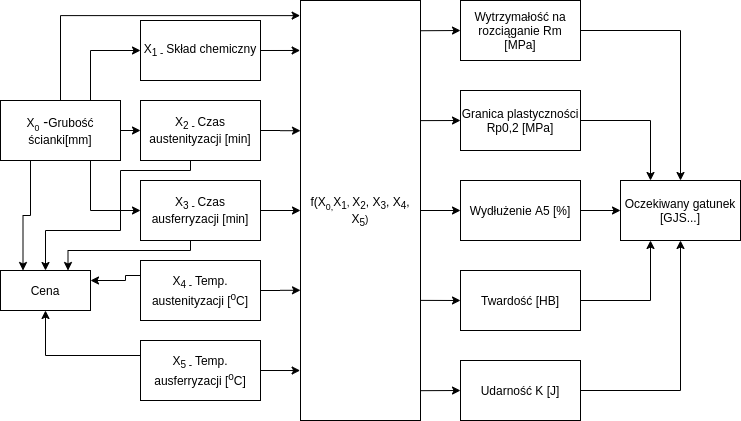
\includegraphics[scale=0.45]{images/parametry_produkcji.png}
	\caption {
		 Diagram zależności między parametrami odlewu oraz obróbki cieplnej od właściwości fizycznych odlewu oraz wpływu na cenę detalu.
	}
	\label{fig:parametry}
\end{figure}

Na diagramie znajduje się blok przedstawiający model predykcyjny\linebreak$f(X_{0},X_{1},X_{2},X_{3},X_{4},X_{5})$, (parametry $X_{i}$ zostały opisane na diagramie), który ma za zadanie przewidywać właściwości mechaniczne wyrobu. Zakłada się, że możliwe jest stworzenie takiego modelu, dzięki któremu będzie możliwe otrzymywanie informacji o gatunku żeliwa dla wybranych parametrów procesu produkcji odlewu. Wzorując się na wymiarach wejściowych modeli przedstawionych w \cite{YESCAS2001162}, czas ausferrytyzacji zostanie także przedstawiony jako wartość logarytmu o podstawie 10 z wartości czasu w sekundach.

Bazując na przygotowanych przez ekspertów tabelach opisujących wpływ poszczególnych parametrów wytopu na cenę gotowego detalu (zakładając wagę detalu 1kg), została opracowana funkcja kosztu:

\begin{equation}
   C(CC, HTP) = \Big(1+cost\_inc\_cc(CC) + \sum_{htp \in HTP} cost\_inc\_htp(htp)\Big) \cdot avg\_iron\_cost 
\end{equation}
gdzie:
\begin{itemize}
    \item \textit{CC} (chemical composition) - zbiór parametrów składu chemicznego wytopu
    \item \textit{HTP} (heat treatment parameters) - zbiór parametrów obróbki cieplnej, który zawiera następujące elementy:
    \begin{itemize}
        \item temperatura austenityzacji,
        \item czas austenityzacji,
        \item temperatura ausferrytyzacji,
        \item czas ausferrytyzacji,
    \end{itemize}
    \item \textit{cost\_inc\_cc} (cost increase) - funkcja zwracająca procent wzrostu kosztu w zależności od składu chemicznego (dokładnie od zawartości niklu, miedzi i molibdenu),
    \item \textit{cost\_inc\_htp} (cost increase) - funkcja zwracająca procent wzrostu kosztu w zależności od wartości parametru obróbki termicznej,
    \item \textit{avg\_iron\_cost} (average iron cost) - średnia cena żeliwa sferoidalnego,
    \item \textit{htp} - parametr ze zbioru parametrów obróbki cieplnej np. temp. austenityzacji, 880\degree C,
    \item \textit{base\_cost} - koszt bazowy np. 61 zł.
\end{itemize}

\section{Funkcja jakości}
Przegląd różnych badań właściwości żeliwa ADI pokazuje, że badania te często są przeprowadzane w postaci eksperymentów, w~których eksplorowane są niestosowane w masowej produkcji zestawy parametrów. Takie zestawy parametrów mogą być uważane za mało wiarygodne przez użytkownika systemu. W tym celu zaproponowana została funkcja określająca jakość parametrów dla zdefiniowanych przez użytkownika nominalnych zakresów prametrów oraz wag tych parametrów. Wartość takiej funkcji będzie określała jak bardzo parametry zwrócone przez system są zgodne z oczekiwaniami użytkownika. Funkcja została zdefiniowana w następującej postaci:
\begin{equation}
     Q(P) = \sum_{p \in P} \big(in\_range(p) \cdot w_p\big) 
\end{equation}

gdzie:
\begin{itemize}
    \item \textit{P} - zbiór parametrów produkcji (skład chemiczny, obróbka cieplna)
    \item \textit{p} - parametr ze zbioru P
    \item \textit{in\_range} - funkcja określająca, czy wartość danego parametru mieści się w przedziale zdefiniowanym przez użytkownika
    \item \textit{w\textsubscript{p}} - waga parametru p, zdefiniowana przez użytkownika
\end{itemize}

\section{Optymalizacja heurystyczna}\label{sec:heur-opt}
W pracy zakładane jest użycie różnych algorytmów heurystycznych z dziedziny optymalizacji jednokryterialnej. Zachodzi także potrzeba zdefiowania zbioru parametrów, które będą eksplorowane za pomocą algorytmów.

\subsection{Zbiór parametrów}\label{sec:param_set}
Budowa zbioru parametrów produkcji będzie opierać się na:
\begin{itemize}
    \item przyjętych przez wytwórców żeliwa możliwych zmianach parametrów obróbki cieplnej tj. zmiany temperatur o +/- 5 stopni Celsjusza, zmiany czasów o +/- 15 minut,
    \item założeniu, że zbiór składów chemicznych jest skończony i ograniczony do składów, które wystąpiły w trakcie uczenia i testowania modelu predykcyjnego oraz składów wprowadzonych przez użytkownika,
    \item minimalnych i maksymalnych wartości parametrów produkcji, jakie wystąpiły podczas uczenia i testowania modelu predykcyjnego.
\end{itemize}

\subsection{Optymalizacja jednokryterialna}\label{sec:opt}
W przypadku użycia algorytmów optymalizacji jednokryterialnej zachodzi potrzeba sprowadzenia zdefiniowanych poprzednio kryteriów tj. kosztu i jakości, do jednego kryterium. Jednym ze sposobów na dokonanie takiego sprowadzenia, jest użycie skalaryzacji ważonej, która polega na znormalizowaniu wartości kryteriów do takiego samego zakresu wartości np. [0,1], a następnie zsumowaniu tych wartości przemnożonych przez wagi tych kryteriów.

W takim podejściu zostanie przyjęte, że to użytkownik wprowadza wagi kryteriów optymalizacyjnych. Problem skalaryzacji ważonej dla znormalizowanych kryteriów ceny i~jakości wygląda następująco:
\begin{equation}
     \min_{(CC,HTP) \in X} QC\Big(C\_norm(CC,HTP),1-Q\_norm(CC \cup HTP),\theta\Big) 
\end{equation}
gdzie:
\begin{itemize}
    \item CC - zbiór parametrów składu chemicznego wytopu,
    \item HTP - zbiór parametrów obróbki cieplnej,
    \item X - zbiór wszystkich możliwych parametrów,
    \item C\_norm - znormalizowana wartość funkcji kosztu,
    \item Q\_norm - znormalizowana wartość funkcji jakości,
    \item $\theta$ - zbiór wag kryteriów kosztu i jakości ,
    \item QC - funkcja następującej postaci:
    \begin{equation}
        QC(X_1, X_2, \theta) = X_1\cdot\theta(X_1) + X_2\cdot\theta(X_2)
    \end{equation}
\end{itemize}

Przedstawiony powyżej problem polega na minimalizacji funkcji QC dla parametrów produkcji. Aby rozwiązania znajdowane przez algorytm były poprawne, należy wprowadzić ograniczenia wynikające z gatunku wymaganego przez klienta. Są one zdefiniowane we wspomnianej już wcześniej normie EN-PN 1564, w której znajdują się minimalne (i~ maksymalne dla twardości) wartości właściwości mechanicznych w zależności od oczekiwanej grubości detalu. 

W celu sprawdzenia, czy dla danych parametrów produkcji otrzymamy oczekiwane przez normę wartości mechaniczne, użyty zostanie zbudowany model predykcyjny opisany w podrozdziale  \ref{sec:model}. Model dla podanych parametrów zwróci przewidywane właściwości mechaniczne i na ich podstawie możliwe będzie sprawdzenie, czy będą one spełniały warunki wymagane przez normę.

\subsection{Wybrane algorytmy i metodologia ich porównania}\label{sec:algos}
Dla celów badawczych zostaną wybrane różne algorytmy heurystyczne służące do optymalizacji jednokryterialnej.

W celu porówniania działania algorytmów, zostanie przeprowadzony test polegający na przeprowadzeniu procesu optymalizacji dla różnych ograniczeń czasowych, w których mierzone i porównywane będą następujace wartości:
\begin{itemize}
    \item liczba przeliczeń funkcji QC,
    \item liczba przewidywań wartości właściwości mechanicznych, które w rezultacie będą eliminować wybrane parametry,
    \item najniższą wartość funkcji QC.
\end{itemize}

\subsubsection{Algorytmy optymalizacji jednokryterialnej}
Do przeprowadzenia badań w kontekście optymalizacji jednokryterialnej zostały wybrane algorytmy z dziedziny lokalnego przeszukiwania:
\begin{itemize}
    \item Stochastic Hill Climbing - stochastyczne wspinanie,
    \item Hill Climbing - podstawowa wersja wspinania,
    \item Tabu search,
    \item Metropolis search,
    \item Parallel tempering - współbieżne szukanie za pomocą wielu instancji Metropolis Search z różnymi temperaturami.
\end{itemize}

% \section{System agentowy}
% \label{system_agentowy}
% Na potrzeby wspomagania decyzji zostanie stworzony system agentowy o koncepcyjnej strukturze znajdujacej się na rys. \ref{fig:system_agentowy}.

% \begin{figure}[h]{}
% 	\centering
% 	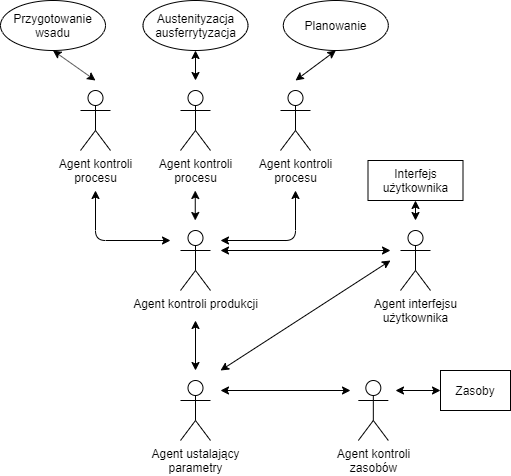
\includegraphics[scale=0.6]{images/system_agentowy.png}
% 	\caption {
% 		 Koncepcyjny schemat systemu agentowego na potrzeby wspomagania decyzji.
% 	}
% 	\label{fig:system_agentowy}
% \end{figure}

% Na schemacie można wyróżnić następujące elementy:
% \begin{itemize}
%     \item procesy, a w nich:
%     \begin{itemize}
%         \item \textbf{proces planowania} - w trakcie trwania tego procesu zbierane są dane o wymaganiach co do realizowanego zamównienia (masa detalu, ilość sztuk, wymagany gatunek) przez agenta kontroli procesu
%         \item \textbf{proces obróbki cieplnej} (austenityzacja, ausferrytyzacja) - wykonywany dla danych dostarczonych przez agenta kontroli procesu (temperatury i czasy trwania poszczególnych etapów obróbki)
%         \item \textbf{proces przygotowania wsadu} - wykonywany dla danych dostarczonych przez agenta kontroli procesu (skład wytopu)
%     \end{itemize}
%     \item agenci, a w nich:
%     \begin{itemize}
%         \item \textbf{Agent kontroli procesu} - agent zajmujący się bezpośrednią komunikacją z procesem (zbiera lub dostarcza dane)
%         \item \textbf{Agent kontroli produkcji} - agent zajmujący się kontrolą produkcji poszczególnych procesów i zarządzaniem danych, które od nich otrzymuje.
%         \item \textbf{Agent interfejsu użytkownika} - agent zajmujący się komunikacją z: użytkownikiem poprzez interfejs użytkownika; agentem kontroli produkcji; agentem ustalającym parametry
%         \item \textbf{Agent ustalający parametry} - na podstawie informacji ustalonych podczas procesu planowania, przeszukuje za pomocą algorytmów heurystycznych przestrzeń rozwiązań w celu zminimalizowania kosztu przy jednoczesnym spełnieniu wymaganej jakości
%         \item \textbf{Agent kontroli zasobów} - agent dostarczający informację o dostępnych zasobach (ilości składowych wytopów, możliwych czasach użycia pieców służących do obróbki cieplnej).
%     \end{itemize}
%     \item elementy zewnętrzne:
%     \begin{itemize}
%         \item interfejs użytkownika
%         \item zasoby
%     \end{itemize}
% \end{itemize}

\section{Koncepcja wspomagania decyzji}\label{sec:dec-sup-sys-concept}
Założone zostało stworzenie systemu wykorzystującego opisane powyżej elementy, tj, optymalizacja kryteriów jakości i kosztu oraz modele predykcyjne, dla potrzeb wspomagania decyzji o wyborze składu wytopu oraz parametrów obróbki cieplnej dla żądanego gatunku oraz określonych zakresów wiarygodności parametrów. 

Użytkownik systemu będzie miał za zadanie wprowadzać niezbędne informacje za pomocą interfejsu graficznego. Informacjami wprowadzanymi przez użytkownika będą:
\begin{itemize}
    \item wymagany gatunek odlewu,
    \item grubość odlewu,
    \item liczba sztuk detalu oraz jego waga,
    \item wagi kryteriów kosztu i jakości,
    \item zakresy wiarygodności parametrów oraz ich wagi,
    \item maksymalny czas szukania rozwiazania.
\end{itemize}
Dodatkowymi parametrami związanymi z wyliczaniem wartości funkcji kosztu są:
\begin{itemize}
    \item ceny niklu, miedzi, molibdenu,
    \item średnia cena żeliwa ADI.
\end{itemize}
W odpowiedzi system będzie zwracał rozwiązanie zawierające następujące informacje:
\begin{itemize}
    \item skład chemiczny wytopu,
    \item parametry obróbki cieplnej,
    \item wartość funkcji kosztu,
    \item wartość funkcji jakości.
\end{itemize}

Została opracowana abstrakcyjna architektura omówionej koncepcji systemu. Jej schemat został przedstawiony na rysunku \ref{fig:abst-arch}. Dla przejrzystości tego schematu, pominięte zostały opisy danych przekazywanych między obiektami systemu.
\begin{figure}[ht]{}
	\centering
	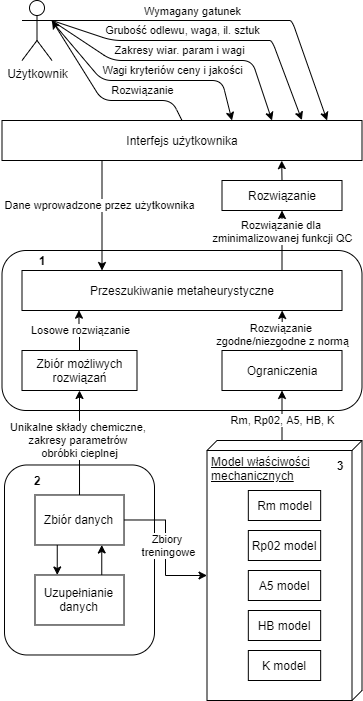
\includegraphics[scale=1]{images/system_wspomagania_decyzji-new.png}
	\caption {
		 Abstrakcyjna architektura systemu wspomagania decyzji.
	}
	\label{fig:abst-arch}
\end{figure}

\FloatBarrier

Opis bloków przedstawionych na rys. \ref{fig:abst-arch}:
\begin{itemize}
    \item Interfejs użytkownika - warstwa oddzielająca użytkownika od systemu za pomocą której użytkownik będzie w stanie wprowadzić dane niezbędne do przeprowadzenia czynności skutkujących dostarczeniem rozwiązania/rozwiązań,
    \item Blok nr 1:
    \begin{itemize}
        \item Przeszukiwanie metaheurystyczne - moduł odpowiedzialny za przeszukiwanie przestrzeni rozwiązań w celu optymalizacji parametrów produkcji poprzez minimalizację funkcji QC,
        \item Zbiór możliwych rozwiązań - element systemu zawierający składowe pozwalające na zbudowanie przestrzeni rozwiązań, która zostanie użyta przez moduł przeszukiwania, 
        \item Ograniczenia - reprezentują wymagania jakie narzuca norma na właściwości mechaniczne wytopu, który byłby wytworzony korzystając z rozwiązania zwracanego przez system.
    \end{itemize}
    \item Blok nr 2:
    \begin{itemize}
        \item Zbiór danych - dane zebranych z artykułów,
        \item Uzupełnianie danych - moduł umożliwiający uzupełnienie brakujących danych w zbiorze danych. 
    \end{itemize}
    \item Model właściwości mechanicznych (blok nr 3) - dostarcza wartości właściwości mechanicznych dla danego rozwiązania,
    \item Rozwiązanie - reprezentuje odpowiedź, jaka zostanie zwrócona użytkownikowi (może zawierać zarówno jedno jak i wiele rozwiązań dla zminimalizowanej funkcji QC).
\end{itemize}



% \bt

% \section{Method 1}

% \bt

% \section{Method 2}

% \bt 

% \section{Method 3}

% Some nice matrices...

% \begin{equation}
% 	A = \begin{bmatrix}
% 		1 &    &    &    &    &    &    & \\
% 		1 & -2 &  1 &    &    &    &    & \\
% 		  &  1 & -2 &  1 &    &    &    & \\
% 		  &    &  1 & -2 &  1 &    &    & \\
% 		  &    &    &  1 & -2 &  1 &    & \\
% 		  &    &    &    &  1 & -2 &  1 & \\
% 		  &    &    &    &    &    &  1 & \\
% 	\end{bmatrix}
% 	\hspace{1cm}
% 	B = \begin{bmatrix}
% 		0 \\
% 		4 \\
% 		4 \\
% 		4 \\
% 		4 \\
% 		4 \\
% 		0
% 	\end{bmatrix}
% \end{equation}

% Some nice diagrams...

% \newcommand{\cv}[1]{ % column vector
% 	$\begin{bmatrix} #1 \end{bmatrix}$
% }
% \newcommand{\Cv}[1]{ { \cv{#1} } } % shortcut for tree leaves
% \newcommand{\elim} { $\xrightarrow{E}$ }
% \newcommand{\merge} { $\xrightarrow{M}$ }
% \newcommand{\xtract} { $\xrightarrow{X}$ }

% \begin{figure}[H]
% 	\centering
% 	\caption{Elimination tree for multifrontal solver}
% 	\label{fig:mfs-elim-tree}
% 	\begin{forest}
% 		for tree = {
% 			draw,
% 			edge={<-, line width=2pt},
% 			minimum height=2cm,
% 			anchor=north,
% 			align=center,
% 			child anchor=north
% 		},
% 		[ { \merge \cv{x_1 \\ x_5 \\ x_7} \elim \cv{x_1 \\ x_7 } }
% 			[ { \merge \cv{x_1 \\ x_3 \\ x_5} \elim \cv{x_1 \\ x_5} }
% 				[ { \merge \cv{x_1 \\ x_2 \\ x_3} \elim \cv{x_1 \\ x_3} }
% 					[ \Cv{x_1 \\ x_2} ]
% 					[ \Cv{x_2 \\ x_3} ]
% 				]
% 				[ { \merge \cv{x_3 \\ x_4 \\ x_5} \elim \cv{x_3 \\ x_5} }
% 					[ \Cv{x_3 \\ x_4} ]
% 					[ \Cv{x_4 \\ x_5} ]
% 				]
% 			]
% 			[ { \merge \cv{x_5 \\ x_6 \\ x_7} \elim \cv{x_5 \\ x_7} }
% 				[ \Cv{x_5 \\ x_6} ]
% 				[ \Cv{x_6 \\ x_7} ]
% 			]
% 		]
% 	\end{forest}
% \end{figure}

% \pagebreak

% Some nice algorithms...

% \newcommand{\U}{\mathcal{U}}

% \begin{algorithm}
% \caption{One iteration of the double-grid algorithm}
% \label{alg:two-grid}

% \begin{algorithmic}

% 	\State Compute the solution $\U^C$ on the coarse mesh
% 	\State Split each element of the coarse mesh, thus obtaining the fine mesh
% 	\State Compute the solution $\U^F$ on the fine mesh

% 	\For{\textbf{each} coarse mesh element $\eps_i$}
% 		\LineComment{$\rho_i$ is the relative error}
% 		\State $ \rho_i \gets \left|
% 				\frac {
% 					\U^F_i - \U^C_i
% 				} {
% 					\U^F_i
% 				}
% 			\right| $
% 	\EndFor

% 	\State $\rho_{max} \gets$ $max_i(\rho_i)$

% 	\For{\textbf{each} element $\eps_i$}
% 		\If {$ \rho_i > \tau \cdot \rho_{max} $}
% 			\State adapt the $\eps_i$ element (split into two halves)
% 		\EndIf
% 	\EndFor

% \end{algorithmic}
% \end{algorithm}

% \pagebreak

% Some nice figures...

% \begin{figure}[H]
% 	\centering

% 	\caption[Double-grid h-adaptation strategy, steps 1-2] {
% 		Steps 1-5 of the double-grid h-adaptation strategy, quadratic B-splines
% 	}
% 	\label{fig:h-adapt-two-grid}

	

% 	\begin{subfigure}[h]{1.0\textwidth}
% 		\centering
% 		\includegraphics[scale=0.2]{frog.jpg}
% 		\caption{
% 			Step 2.
% 			Since the maximal error multiplied by $\tau$ (here set to 20\%) were lower than the error on any element,
% 			the algorithm halved all four elements after step 1.
% 		}
% 		\label{fig:h-adapt-two-grid-2}
% 	\end{subfigure}
% \end{figure}


% \begin{figure}[H]
% 	\ContinuedFloat % continue from previous page
% 	\caption[Double-grid h-adaptation strategy, steps 3-4]{} % for subcaption package to ensure proper numbering

% 	\begin{subfigure}[h]{1.0\textwidth}
% 		\centering
% 		\includegraphics[scale=0.2]{frog.jpg}
% 		\caption{
% 			Step 3.
% 			The extreme left and right elements did not get refined after the step 2.
% 		}
% 		\label{fig:h-adapt-two-grid-3}
% 	\end{subfigure}

% 	\begin{subfigure}[h]{1.0\textwidth}
% 		\centering
% 		\includegraphics[scale=0.2]{frog.jpg}
% 		\caption{
% 			Step 4
% 		}
% 		\label{fig:h-adapt-two-grid-4}
% 	\end{subfigure}
% \end{figure}


